\section{Analyse und Bewertung der Teilprozesse und Stakeholder}

In diesem Kapitel werden die Stakeholder des neu zu entwickelnden Systems für die Anrechnung von Studien – und Prüfungsleistungen behandelt. Dabei wird auf deren Rolle im bisherigen Prozess eingegangen und die Veränderungen durch eine mögliche Einführung eines neuen Systems beschrieben. Das neue System hat vier Stakeholder: die Mitarbeiter des Prüfungsamtes, die Mitglieder des Prüfungsausschusses, die Studierenden und die zuständige IT-Abteilung.

\resizebox{\textwidth}{!}{%
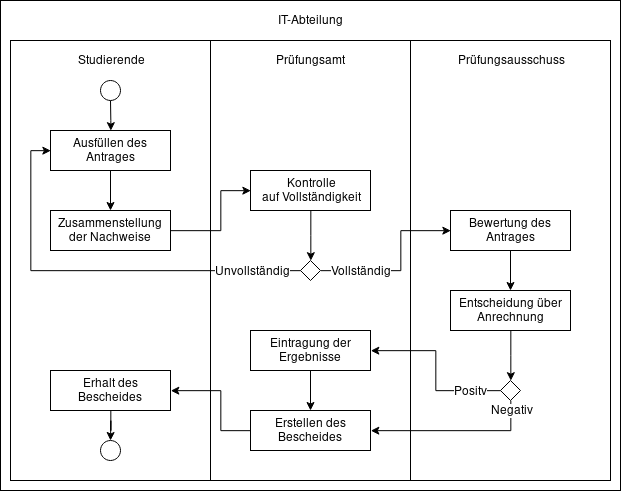
\includegraphics{../../images/analoger_prozess.png}%
}